\documentclass[../../main.tex]{subfiles}

\graphicspath{{../../image/}{../../figure/}}

\begin{document}

\section{生成分类器}\label{section:ch05-生成分类器}

本节将从概率的角度分析分类问题并展示如何通过对数据分布进行简单的假设来建立具有线性决策边界的模型。我们已经讨论过分类的判别法和生成法的区别（参见\cref{subsection:ch05-推理和决策}）。在这里，我们将采用对类-条件概率密度$p(\boldsymbol{x}\mid C_k)$以及类的先验概率$p(C_k)$进行建模的生成法，然后通过 Bayes 定理使用这些量来计算后验概率$p(C_k\mid\boldsymbol{x})$。

首先考虑二分类问题。$C_1$类的后验概率可以写成

\begin{align}
  p(C_1\mid\boldsymbol{x})&=\frac{p(\boldsymbol{x}\mid C_1)\,p(C_1)}{p(\boldsymbol{x}\mid C_1)\,p(C_1)+p(\boldsymbol{x}\mid C_2)\,p(C_2)}\nonumber\\
  &=\frac{1}{1+\exp(-a)}=\sigma(a)
  \label{align:ch05-二类后验sigmoid}
\end{align}

其中：

\begin{align}
  a=\ln\frac{p(\boldsymbol{x}\mid C_1)\,p(C_1)}{p(\boldsymbol{x}\mid C_2)\,p(C_2)}
  \label{align:ch05-预激活对数比}
\end{align}

\begin{definition}[logistic sigmoid 函数]\label{definition:ch05-logistic-sigmoid}
函数
\begin{align}
  \sigma(a)=\frac{1}{1+\exp(-a)}
  \label{align:ch05-sigmoid定义}
\end{align}
称为 logistic sigmoid 函数。
\end{definition}

logistic sigmoid 函数$\sigma(a)$如\cref{figure:ch05-sigmoid与probit}所示，这类函数有时也称“压缩函数”，因为它们能将整个实轴映射到一个有限区间内。logistic sigmoid 函数$\sigma(a)$在许多分类算法中发挥着重要作用，其满足如下对称性：

\begin{align}
  \sigma(-a)=1-\sigma(a)
  \label{align:ch05-sigmoid对称}
\end{align}

\begin{figure}[htbp]
  \centering
  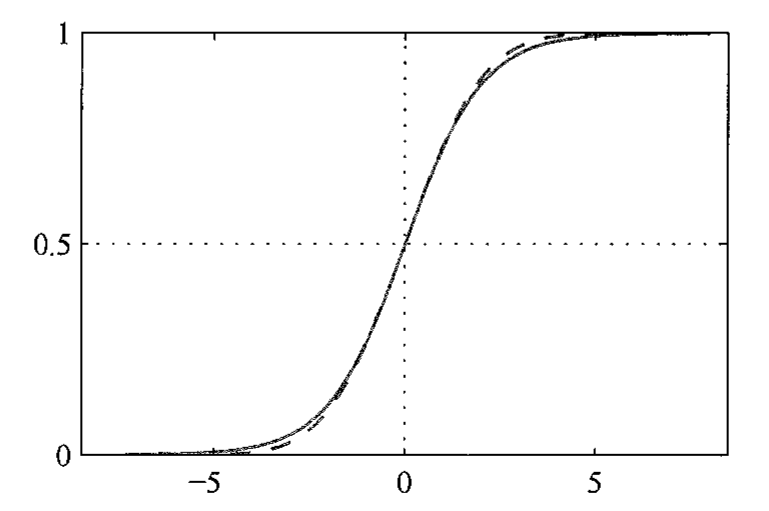
\includegraphics[width=0.52\textwidth]{ch05-fig5-12-sigmoid-probit.png}
  \caption{红色实线表示由\eqref{align:ch05-sigmoid定义}定义的 logistic sigmoid 函数$\sigma(a)$，蓝色虚线表示$\lambda^{2}=\pi/8$时的缩放 probit 函数$\Phi(\lambda a)$，其中$\Phi(a)$由\eqref{align:ch05-probit函数}定义。选择缩放因子$\pi/8$是为了使$a=0$时这两条曲线的导数相等}
  \label{figure:ch05-sigmoid与probit}
\end{figure}

% SUPPLEMENT: parent=definition:ch05-logistic-sigmoid; kind=motivation; location=紧随其后的 remark（重构新增）
\begin{remark}（重构新增）
\cref{definition:ch05-logistic-sigmoid}中的$\sigma$把$\mathbb{R}$双射到$(0,1)$，其反函数即下面的 logit 函数，因此它是“把线性函数的输出转换为概率”的最自然选择之一。\eqref{align:ch05-sigmoid对称}可由定义直接验证：$\sigma(-a)=1/(1+\exp a)=\exp(-a)/(1+\exp(-a))=1-\sigma(a)$。该对称性说明$\sigma(0)=1/2$，即“两个类概率相等”对应预激活为0，这正是决策面的位置。$\sigma$的导数满足$\sigma'(a)=\sigma(a)(1-\sigma(a))$（见\cref{proposition:ch05-sigmoid导数}），这一性质使交叉熵的梯度化简为“误差乘以特征”，是\cref{subsection:ch05-logistic回归}的出发点。注意$\sigma$没有封闭形式的反函数初等表达式以外的简化，其逆就是 logit；在选择激活函数时，logistic 与 probit 的差别主要在于尾部衰减速度（见\cref{subsection:ch05-probit回归}）。
\end{remark}

logistic sigmoid 函数$\sigma(a)$的倒数为

\begin{align}
  a=\ln\left(\frac{\sigma}{1-\sigma}\right)
  \label{align:ch05-logit}
\end{align}

\begin{definition}[logit 函数]\label{definition:ch05-logit}
\eqref{align:ch05-logit}定义的函数称为 logit 函数。它表示两个类的概率之比的对数$\ln[p(C_1\mid\boldsymbol{x})/p(C_2\mid\boldsymbol{x})]$，也称对数几率。
\end{definition}

% SUPPLEMENT: parent=definition:ch05-logit; kind=motivation; location=紧随其后的 remark（重构新增）
\begin{remark}（重构新增）
“几率”指事件发生与不发生的概率之比，logit 即几率的对数，故 logit 把$(0,1)$映到$\mathbb{R}$，与$\sigma$互为反函数。\eqref{align:ch05-二类后验sigmoid}与\eqref{align:ch05-预激活对数比}合起来说明：后验概率的对数几率恰等于两个“类-条件密度乘先验”之比的对数。这一等式的用处在于，只要该对数比值是$\boldsymbol{x}$的线性函数，后验就自动具有 logistic 形式；$\boldsymbol{x}$本身的分布形式并不重要，重要的只是比值的函数形式。这就是下一小节要研究的“线性”从何而来的问题。
\end{remark}

请注意，在\eqref{align:ch05-二类后验sigmoid}中，我们只是以等价形式重写了后验概率，因此 logistic sigmoid 函数的出现似乎是人为的。不过，只要$a(\boldsymbol{x})$具有约束函数形式，它就具有重要意义。我们很快就会讨论$a(\boldsymbol{x})$是$\boldsymbol{x}$的线性函数的情况，在此情况下，后验概率受广义线性模型的控制。

如果存在$K>2$个类，则有

\begin{align}
  p(C_k\mid\boldsymbol{x})&=\frac{p(\boldsymbol{x}\mid C_k)\,p(C_k)}{\sum_j p(\boldsymbol{x}\mid C_j)\,p(C_j)}\nonumber\\
  &=\frac{\exp(a_k)}{\sum_j\exp(a_j)}
  \label{align:ch05-softmax后验}
\end{align}

这就是归一化指数（normalized exponential），它可以视为 logistic sigmoid 函数的多类泛化。在这里，量$a_k$由下式定义：

\begin{align}
  a_k=\ln\bigl(p(\boldsymbol{x}\mid C_k)\,p(C_k)\bigr)
  \label{align:ch05-预激活定义}
\end{align}

\begin{definition}[归一化指数与 softmax 函数]\label{definition:ch05-归一化指数}
对实数$a_1,\cdots,a_K$，由
\begin{align}
  y_k=\frac{\exp(a_k)}{\sum_j\exp(a_j)},\qquad k=1,\cdots,K,
\end{align}
定义的变换称为归一化指数（normalized exponential），也称 softmax 函数，其中$a_k$称为预激活。
\end{definition}

归一化指数也叫 softmax 函数，因为它代表了$\max$函数的平滑版本。如果$a_k\gg a_j$，则对于所有$j\neq k$，$p(C_k\mid\boldsymbol{x})\approx 1$且$p(C_j\mid\boldsymbol{x})\approx 0$。

% SUPPLEMENT: parent=definition:ch05-归一化指数; kind=motivation; location=紧随其后的 remark（重构新增）
\begin{remark}（重构新增）
softmax 与 logistic sigmoid 的关系是：$K=2$时，令$a=a_1-a_2$，则$y_1=\exp(a_1)/(\exp(a_1)+\exp(a_2))=1/(1+\exp(-a))=\sigma(a)$，故 sigmoid 是 softmax 的二类特例。softmax 的一个重要性质是平移不变性：把所有$a_k$同时加上常数$c$，$y_k$不变，因此\eqref{align:ch05-softmax后验}中的$a_k$只需确定到一个共同的加性常数，这也说明多类模型的参数存在冗余（见\cref{subsection:ch05-多类logistic回归}）。另一个性质是$\sum_k y_k=1$且$y_k>0$，因此输出可以直接解释为概率，这与最小二乘分类的输出不同（见\cref{subsection:ch05-最小二乘分类}）。“softmax”之名来自它是对$\max$的平滑近似：当某个$a_k$远大于其他时，$y_k\to1$，其余趋于0。
\end{remark}

接下来研究选择特定形式的类-条件概率密度的后果。首先讨论连续输入变量$\boldsymbol{x}$，然后简要讨论离散输入。

\subsection{连续输入}\label{subsection:ch05-连续输入}

假设类-条件概率密度是 Gauss 密度。我们将探讨由此产生的后验概率形式。假设所有类共享相同的协方差矩阵$\boldsymbol{\Sigma}$，则$C_k$类的密度为

\begin{align}
  p(\boldsymbol{x}\mid C_k)=\frac{1}{(2\pi)^{D/2}\lvert\boldsymbol{\Sigma}\rvert^{1/2}}\exp\left\{-\frac{1}{2}(\boldsymbol{x}-\boldsymbol{\mu}_k)^{\mathsf{T}}\boldsymbol{\Sigma}^{-1}(\boldsymbol{x}-\boldsymbol{\mu}_k)\right\}
  \label{align:ch05-Gauss类条件}
\end{align}

假设我们有两个类。根据\eqref{align:ch05-二类后验sigmoid}与\eqref{align:ch05-预激活对数比}，可得

\begin{align}
  p(C_1\mid\boldsymbol{x})=\sigma(\boldsymbol{w}^{\mathsf{T}}\boldsymbol{x}+w_0)
  \label{align:ch05-Gauss后验}
\end{align}

其中

\begin{align}
  \boldsymbol{w}&=\boldsymbol{\Sigma}^{-1}(\boldsymbol{\mu}_1-\boldsymbol{\mu}_2)
  \label{align:ch05-Gauss权重}\\
  w_0&=-\frac{1}{2}\boldsymbol{\mu}_1^{\mathsf{T}}\boldsymbol{\Sigma}^{-1}\boldsymbol{\mu}_1+\frac{1}{2}\boldsymbol{\mu}_2^{\mathsf{T}}\boldsymbol{\Sigma}^{-1}\boldsymbol{\mu}_2+\ln\frac{p(C_1)}{p(C_2)}
  \label{align:ch05-Gauss偏置}
\end{align}

\begin{proposition}[Gauss 类-条件密度导出的线性后验]\label{proposition:ch05-Gauss线性后验}
设两个类的类-条件密度由\eqref{align:ch05-Gauss类条件}给出且共享同一协方差矩阵$\boldsymbol{\Sigma}$（$\boldsymbol{\Sigma}$正定），先验概率满足$p(C_k)>0$。则$C_1$的后验概率具有\eqref{align:ch05-Gauss后验}的形式，其中$\boldsymbol{w}$与$w_0$分别由\eqref{align:ch05-Gauss权重}与\eqref{align:ch05-Gauss偏置}给出。特别地，后验概率的对数几率是$\boldsymbol{x}$的线性函数。
\end{proposition}

\begin{proof}
（重构新增）由\eqref{align:ch05-预激活对数比}，
\begin{align}
  a(\boldsymbol{x})=\ln\frac{p(C_1)}{p(C_2)}+\ln p(\boldsymbol{x}\mid C_1)-\ln p(\boldsymbol{x}\mid C_2)
\end{align}
两个密度的归一化常数相同（因为$\boldsymbol{\Sigma}$相同、维数相同），相减时消去，故只需计算指数部分之差。展开
\begin{align}
  -\frac{1}{2}(\boldsymbol{x}-\boldsymbol{\mu}_1)^{\mathsf{T}}\boldsymbol{\Sigma}^{-1}(\boldsymbol{x}-\boldsymbol{\mu}_1)
  =-\frac{1}{2}\boldsymbol{x}^{\mathsf{T}}\boldsymbol{\Sigma}^{-1}\boldsymbol{x}+\boldsymbol{\mu}_1^{\mathsf{T}}\boldsymbol{\Sigma}^{-1}\boldsymbol{x}-\frac{1}{2}\boldsymbol{\mu}_1^{\mathsf{T}}\boldsymbol{\Sigma}^{-1}\boldsymbol{\mu}_1
\end{align}
对$k=2$有同样的展开。两式相减，二次项$-\frac{1}{2}\boldsymbol{x}^{\mathsf{T}}\boldsymbol{\Sigma}^{-1}\boldsymbol{x}$完全抵消（这正是“共享协方差”假设的作用），剩下
\begin{align}
  a(\boldsymbol{x})=(\boldsymbol{\mu}_1-\boldsymbol{\mu}_2)^{\mathsf{T}}\boldsymbol{\Sigma}^{-1}\boldsymbol{x}-\frac{1}{2}\boldsymbol{\mu}_1^{\mathsf{T}}\boldsymbol{\Sigma}^{-1}\boldsymbol{\mu}_1+\frac{1}{2}\boldsymbol{\mu}_2^{\mathsf{T}}\boldsymbol{\Sigma}^{-1}\boldsymbol{\mu}_2+\ln\frac{p(C_1)}{p(C_2)}
\end{align}
由于$\boldsymbol{\Sigma}^{-1}$对称，$(\boldsymbol{\mu}_1-\boldsymbol{\mu}_2)^{\mathsf{T}}\boldsymbol{\Sigma}^{-1}\boldsymbol{x}=[\boldsymbol{\Sigma}^{-1}(\boldsymbol{\mu}_1-\boldsymbol{\mu}_2)]^{\mathsf{T}}\boldsymbol{x}=\boldsymbol{w}^{\mathsf{T}}\boldsymbol{x}$，其中$\boldsymbol{w}$如\eqref{align:ch05-Gauss权重}；其余与$\boldsymbol{x}$无关的项即$w_0$，如\eqref{align:ch05-Gauss偏置}。再由\cref{definition:ch05-logistic-sigmoid}与\eqref{align:ch05-二类后验sigmoid}，$p(C_1\mid\boldsymbol{x})=\sigma(a(\boldsymbol{x}))$。最后，$a$是$\boldsymbol{x}$的仿射函数，故对数几率$\ln[p(C_1\mid\boldsymbol{x})/p(C_2\mid\boldsymbol{x})]=a(\boldsymbol{x})$是线性的。
\end{proof}

% SUPPLEMENT: parent=proposition:ch05-Gauss线性后验; kind=motivation; location=紧随其后的 remark（重构新增）
\begin{remark}（重构新增）
命题中三个条件各有作用：$\boldsymbol{\Sigma}$正定保证$\boldsymbol{\Sigma}^{-1}$存在且密度归一化；两个类共享$\boldsymbol{\Sigma}$保证二次项相消，这是后验成为线性的关键（若各自协方差不同，见\cref{definition:ch05-二次判别式}）；$p(C_k)>0$保证对数有意义。$w_0$中的$\ln[p(C_1)/p(C_2)]$说明先验只影响偏置，因此改变先验只会使决策面平行移动，而不改变其朝向，这与\cref{proposition:ch05-决策面几何}中“$w_0$决定位置、$\boldsymbol{w}$决定朝向”的解释一致。注意$\boldsymbol{w}$不依赖于先验，也不依赖于$\boldsymbol{x}$；它只由两个均值与共享协方差决定。这一结果的意义在于：不必假设$\boldsymbol{x}$的分布是 Gauss 的，只要两个类的对数密度比是线性的，后验就具有 logistic 形式。
\end{remark}

可以看到，来自 Gauss 密度指数的$\boldsymbol{x}$中的二次项已被消去（缘于共享协方差矩阵的假设），从而在 logistic sigmoid 函数的变量中形成了$\boldsymbol{x}$的线性函数。\cref{figure:ch05-Gauss后验曲面}展示了二维输入空间$\boldsymbol{x}$的结果。由此得出的决策边界对应于后验概率$p(C_k\mid\boldsymbol{x})$恒定的曲面，因此后验概率$p(C_k\mid\boldsymbol{x})$将由$\boldsymbol{x}$的线性函数给出，决策边界在输入空间中是线性的。先验概率$p(C_k)$仅通过偏置参数$w_0$进入，因此先验的变化会使决策边界发生平行位移，更一般地说，这会使恒定后验概率的轮廓发生平行位移。

\begin{figure}[htbp]
  \centering
  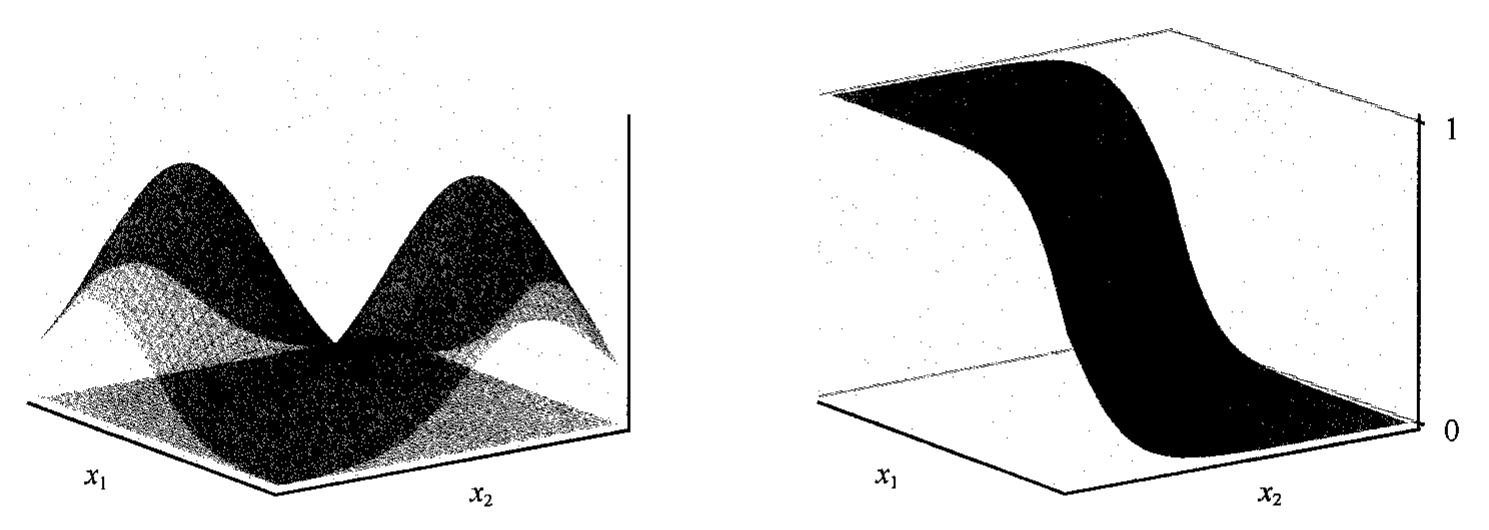
\includegraphics[width=0.92\textwidth]{ch05-fig5-13-gaussian-posterior.png}
  \caption{左图显示了两个类的类-条件概率密度，分别用红色和蓝色表示。右图是相应的后验概率$p(C_1\mid\boldsymbol{x})$，由作用于$\boldsymbol{x}$的线性函数的 logistic sigmoid 函数给出。右图中的面是用红色和蓝色涂色的，红色的比例为$p(C_1\mid\boldsymbol{x})$，蓝色的比例为$p(C_2\mid\boldsymbol{x})=1-p(C_1\mid\boldsymbol{x})$}
  \label{figure:ch05-Gauss后验曲面}
\end{figure}

对于$K$个类的一般情况，后验概率由\eqref{align:ch05-softmax后验}得出。根据\eqref{align:ch05-预激活定义}和\eqref{align:ch05-Gauss类条件}，得出

\begin{align}
  a_k(\boldsymbol{x})=\boldsymbol{w}_k^{\mathsf{T}}\boldsymbol{x}+w_{k0}
  \label{align:ch05-多类预激活}
\end{align}

其中

\begin{align}
  \boldsymbol{w}_k&=\boldsymbol{\Sigma}^{-1}\boldsymbol{\mu}_k
  \label{align:ch05-多类权重}\\
  w_{k0}&=-\frac{1}{2}\boldsymbol{\mu}_k^{\mathsf{T}}\boldsymbol{\Sigma}^{-1}\boldsymbol{\mu}_k+\ln p(C_k)
  \label{align:ch05-多类偏置}
\end{align}

\begin{proposition}[多类情形下的线性预激活]\label{proposition:ch05-多类线性预激活}
设$K$个类的类-条件密度由\eqref{align:ch05-Gauss类条件}给出且共享同一正定协方差矩阵$\boldsymbol{\Sigma}$。则\eqref{align:ch05-预激活定义}中的$a_k$与\eqref{align:ch05-多类预激活}只相差一个与$k$无关的常数；特别地，$a_k(\boldsymbol{x})$可以取为$\boldsymbol{x}$的线性函数，且\eqref{align:ch05-softmax后验}中的后验概率只依赖于这些线性函数。
\end{proposition}

\begin{proof}
（重构新增）由\eqref{align:ch05-预激活定义}，
\begin{align}
  a_k=\ln p(C_k)-\frac{D}{2}\ln(2\pi)-\frac{1}{2}\ln\lvert\boldsymbol{\Sigma}\rvert-\frac{1}{2}(\boldsymbol{x}-\boldsymbol{\mu}_k)^{\mathsf{T}}\boldsymbol{\Sigma}^{-1}(\boldsymbol{x}-\boldsymbol{\mu}_k)
\end{align}
展开二次型得
\begin{align}
  a_k=-\frac{1}{2}\boldsymbol{x}^{\mathsf{T}}\boldsymbol{\Sigma}^{-1}\boldsymbol{x}+\boldsymbol{\mu}_k^{\mathsf{T}}\boldsymbol{\Sigma}^{-1}\boldsymbol{x}-\frac{1}{2}\boldsymbol{\mu}_k^{\mathsf{T}}\boldsymbol{\Sigma}^{-1}\boldsymbol{\mu}_k+\ln p(C_k)-\frac{D}{2}\ln(2\pi)-\frac{1}{2}\ln\lvert\boldsymbol{\Sigma}\rvert
\end{align}
其中第一项与$k$无关。把它与其余与$k$无关的常数项一并记为$c(\boldsymbol{x})$，则$a_k=\boldsymbol{w}_k^{\mathsf{T}}\boldsymbol{x}+w_{k0}+c(\boldsymbol{x})$，其中$\boldsymbol{w}_k=\boldsymbol{\Sigma}^{-1}\boldsymbol{\mu}_k$、$w_{k0}=-\frac{1}{2}\boldsymbol{\mu}_k^{\mathsf{T}}\boldsymbol{\Sigma}^{-1}\boldsymbol{\mu}_k+\ln p(C_k)$。由于 softmax 对每个$a_k$同时加上同一个量不变（见\cref{definition:ch05-归一化指数}后的注记），$c(\boldsymbol{x})$可以从\eqref{align:ch05-softmax后验}中约去，故后验概率由线性函数$\boldsymbol{w}_k^{\mathsf{T}}\boldsymbol{x}+w_{k0}$决定。
\end{proof}

% SUPPLEMENT: parent=proposition:ch05-多类线性预激活; kind=motivation; location=紧随其后的 remark（重构新增）
\begin{remark}（重构新增）
与二分类情形相比，多类情形多了一个“公共二次项”$-\frac{1}{2}\boldsymbol{x}^{\mathsf{T}}\boldsymbol{\Sigma}^{-1}\boldsymbol{x}$：它并不消失，而是对所有$k$相同，因而在 softmax 中被约去。这说明“线性”是相对于 softmax 而言的，而不是说$a_k$本身没有二次项。$\boldsymbol{w}_k=\boldsymbol{\Sigma}^{-1}\boldsymbol{\mu}_k$表明各类的权重向量是均值经同一线性变换得到的，因此当两个类的均值之差与$\boldsymbol{\Sigma}^{-1}$作用后方向相同时，两类之间的决策面与二分类情形一致。$w_{k0}$中的$\ln p(C_k)$说明先验只平移各类的预激活，从而改变决策面到原点的位置。
\end{remark}

可以看到，$a_k(\boldsymbol{x})$是$\boldsymbol{x}$的线性函数，因为共享协方差矩阵消去了二次项。当两个后验概率（后验概率中最大的两个）相等时，就会出现与最小误分类率对应的决策边界，因此决策边界将由$\boldsymbol{x}$的线性函数定义。我们再次得到了一个广义线性模型。

如果我们放宽共享协方差矩阵的假设，并允许每个类-条件概率密度$p(\boldsymbol{x},C_k)$有自己的协方差矩阵$\boldsymbol{\Sigma}_k$，那么先前的二次项消去将不再发生，我们将得到$\boldsymbol{x}$的二次函数，从而产生二次判别式（quadratic discriminant）。线性决策边界和二次方决策边界如\cref{figure:ch05-二次判别边界}所示。

\begin{definition}[二次判别式]\label{definition:ch05-二次判别式}
若各类的类-条件密度为具有各自协方差矩阵$\boldsymbol{\Sigma}_k$的 Gauss 密度，则后验概率的预激活$a_k(\boldsymbol{x})$是$\boldsymbol{x}$的二次函数，相应的决策面为二次曲面。这样的判别式称为二次判别式（quadratic discriminant）。
\end{definition}

\begin{figure}[htbp]
  \centering
  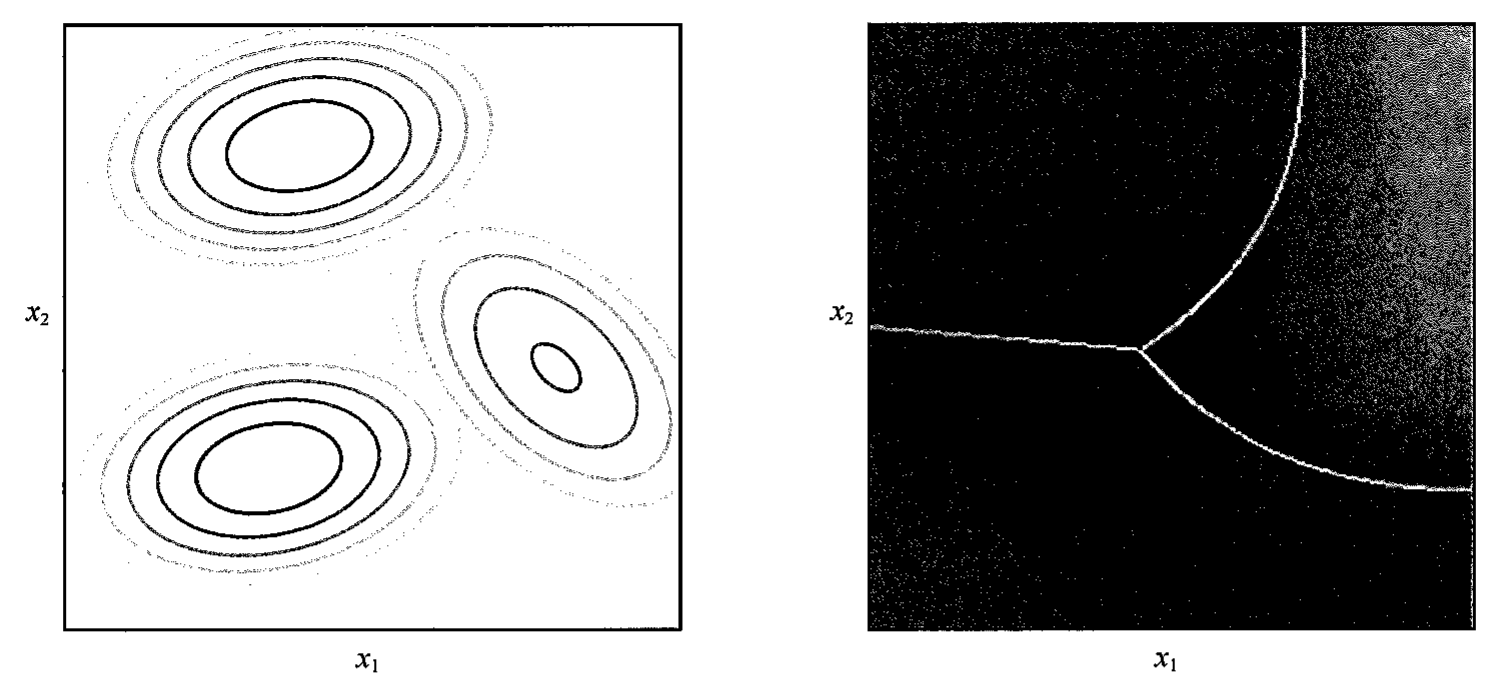
\includegraphics[width=0.95\textwidth]{ch05-fig5-14-quadratic.png}
  \caption{左图显示了三个类的类-条件概率密度，每个类都符合 Gauss 分布，颜色分别为红色、绿色和蓝色，其中红色类和蓝色类的协方差矩阵相同。右图展示了相应的后验概率，其中图像上的每个点都用红、蓝、绿三种颜色按比例着色，分别对应三个类的后验概率。右图还展示了决策边界，请注意，具有相同协方差矩阵的红色类和蓝色类之间的边界是线性的，而红色类和绿色类以及蓝色类和绿色类之间的边界是二次的}
  \label{figure:ch05-二次判别边界}
\end{figure}

% SUPPLEMENT: parent=definition:ch05-二次判别式; kind=motivation; location=紧随其后的 remark（重构新增）
\begin{remark}（重构新增）
二次判别式比线性判别式多出的自由度来自“协方差可以不同”这一放宽：\eqref{align:ch05-多类预激活}的推导中，二次项之所以能约去，靠的是所有类共用同一个$\boldsymbol{\Sigma}$；一旦$\boldsymbol{\Sigma}_k$随$k$变化，二次项$-\frac{1}{2}\boldsymbol{x}^{\mathsf{T}}\boldsymbol{\Sigma}_k^{-1}\boldsymbol{x}$就依赖于$k$，无法在 softmax 中约去，于是$a_k$成为$\boldsymbol{x}$的二次函数。参数数量随之增加（每个类多出$D(D+1)/2$个参数），所需训练数据也更多。二次判别式仍然是“生成式”的：它由类-条件密度的形式推出，而不是直接假设后验的形式。\cref{figure:ch05-二次判别边界}中“红色类与蓝色类的边界是线性的”正是它们协方差相同的结果，这为“共享协方差$\Rightarrow$线性”提供了直观证据。
\end{remark}

\subsection{最大似然解}\label{subsection:ch05-最大似然解}

在为类-条件概率密度$p(\boldsymbol{x}\mid C_k)$指定了一个参数函数形式后，就可以使用最大似然法确定参数值和类的先验概率$p(C_k)$。此时需要一个包含$\boldsymbol{x}$的观测值及其相应类标签的数据集。

假设我们有两个类，每个类都有一个共享协方差矩阵的 Gauss 类-条件概率密度。此外，假设我们有一个数据集$\{\boldsymbol{x}_n,t_n\}$，其中$n=1,\cdots,N$。$t_n=1$表示$C_1$类，$t_n=0$表示$C_2$类。将类的先验概率记为$p(C_1)=\pi$，因此$p(C_2)=1-\pi$。对于属于$C_1$类的数据点$\boldsymbol{x}_n$，我们有$t_n=1$，因此

\begin{align}
  p(\boldsymbol{x}_n,C_1)=p(C_1)\,p(\boldsymbol{x}_n\mid C_1)=\pi\,\mathcal{N}(\boldsymbol{x}_n\mid\boldsymbol{\mu}_1,\boldsymbol{\Sigma})
\end{align}

类似地，对于$C_2$类，我们有$t_n=0$，因此

\begin{align}
  p(\boldsymbol{x}_n,C_2)=p(C_2)\,p(\boldsymbol{x}_n\mid C_2)=(1-\pi)\,\mathcal{N}(\boldsymbol{x}_n\mid\boldsymbol{\mu}_2,\boldsymbol{\Sigma})
\end{align}

似然函数由下式给出：

\begin{align}
  p(\boldsymbol{t},\boldsymbol{X}\mid\pi,\boldsymbol{\mu}_1,\boldsymbol{\mu}_2,\boldsymbol{\Sigma})=\prod_{n=1}^{N}\bigl[\pi\,\mathcal{N}(\boldsymbol{x}_n\mid\boldsymbol{\mu}_1,\boldsymbol{\Sigma})\bigr]^{t_n}\bigl[(1-\pi)\,\mathcal{N}(\boldsymbol{x}_n\mid\boldsymbol{\mu}_2,\boldsymbol{\Sigma})\bigr]^{1-t_n}
  \label{align:ch05-生成似然}
\end{align}

其中$\boldsymbol{t}=(t_1,\cdots,t_N)^{\mathsf{T}}$。按照惯例，最大化似然函数的对数是很方便的。首先考虑关于变量$\pi$的最大值。对数似然函数中取决于变量$\pi$的项为

\begin{align}
  \sum_{n=1}^{N}\bigl\{t_n\ln\pi+(1-t_n)\ln(1-\pi)\bigr\}
  \label{align:ch05-先验项}
\end{align}

设变量$\pi$的导数为0并重新排列，可得

\begin{align}
  \pi=\frac{1}{N}\sum_{n=1}^{N}t_n=\frac{N_1}{N}=\frac{N_1}{N_1+N_2}
  \label{align:ch05-先验ML}
\end{align}

其中，$N_1$表示$C_1$类数据点的总数，$N_2$表示$C_2$类数据点的总数。因此，变量$\pi$的最大似然估计值就是预期中$C_1$类数据点的比例。我们可以很容易地将这一结果扩展到多类情况，在这种情况下，与$C_k$类相关的先验概率的最大似然估计值同样是由归入该类的训练集数据点的比例计算得出的（见\cref{exercise:ch05-13}）。

下面考虑$\boldsymbol{\mu}_1$的最大值。同样，我们可以从对数似然函数中挑出那些取决于$\boldsymbol{\mu}_1$的项：

\begin{align}
  \sum_{n=1}^{N}t_n\ln\mathcal{N}(\boldsymbol{x}_n\mid\boldsymbol{\mu}_1,\boldsymbol{\Sigma})=-\frac{1}{2}\sum_{n=1}^{N}t_n(\boldsymbol{x}_n-\boldsymbol{\mu}_1)^{\mathsf{T}}\boldsymbol{\Sigma}^{-1}(\boldsymbol{x}_n-\boldsymbol{\mu}_1)+\text{const}
  \label{align:ch05-均值项}
\end{align}

设$\boldsymbol{\mu}_1$的导数为0并重新排列，可得

\begin{align}
  \boldsymbol{\mu}_1=\frac{1}{N_1}\sum_{n=1}^{N}t_n\boldsymbol{x}_n
  \label{align:ch05-均值ML1}
\end{align}

此为归入$C_1$类的所有输入向量$\boldsymbol{x}_n$的平均值。经过类似的论证，$\boldsymbol{\mu}_2$的相应结果的计算公式为

\begin{align}
  \boldsymbol{\mu}_2=\frac{1}{N_2}\sum_{n=1}^{N}(1-t_n)\boldsymbol{x}_n
  \label{align:ch05-均值ML2}
\end{align}

此为归入$C_2$类的所有输入向量$\boldsymbol{x}_n$的平均值。

最后，考虑共享协方差矩阵$\boldsymbol{\Sigma}$的最大似然解。选出对数似然函数中依赖于$\boldsymbol{\Sigma}$的项：

\begin{align}
  &-\frac{1}{2}\sum_{n=1}^{N}t_n\ln\lvert\boldsymbol{\Sigma}\rvert-\frac{1}{2}\sum_{n=1}^{N}t_n(\boldsymbol{x}_n-\boldsymbol{\mu}_1)^{\mathsf{T}}\boldsymbol{\Sigma}^{-1}(\boldsymbol{x}_n-\boldsymbol{\mu}_1)\nonumber\\
  &\quad-\frac{1}{2}\sum_{n=1}^{N}(1-t_n)\ln\lvert\boldsymbol{\Sigma}\rvert-\frac{1}{2}\sum_{n=1}^{N}(1-t_n)(\boldsymbol{x}_n-\boldsymbol{\mu}_2)^{\mathsf{T}}\boldsymbol{\Sigma}^{-1}(\boldsymbol{x}_n-\boldsymbol{\mu}_2)\nonumber\\
  &=-\frac{N}{2}\ln\lvert\boldsymbol{\Sigma}\rvert-\frac{N}{2}\operatorname{tr}\bigl\{\boldsymbol{\Sigma}^{-1}\boldsymbol{S}\bigr\}
  \label{align:ch05-协方差项}
\end{align}

其中

\begin{align}
  \boldsymbol{S}&=\frac{N_1}{N}\boldsymbol{S}_1+\frac{N_2}{N}\boldsymbol{S}_2
  \label{align:ch05-共享协方差}\\
  \boldsymbol{S}_1&=\frac{1}{N_1}\sum_{n\in C_1}(\boldsymbol{x}_n-\boldsymbol{\mu}_1)(\boldsymbol{x}_n-\boldsymbol{\mu}_1)^{\mathsf{T}}
  \label{align:ch05-类协方差1}\\
  \boldsymbol{S}_2&=\frac{1}{N_2}\sum_{n\in C_2}(\boldsymbol{x}_n-\boldsymbol{\mu}_2)(\boldsymbol{x}_n-\boldsymbol{\mu}_2)^{\mathsf{T}}
  \label{align:ch05-类协方差2}
\end{align}

利用 Gauss 分布最大似然解的标准结果，我们可以得出$\boldsymbol{\Sigma}=\boldsymbol{S}$，它表示分别与两个类相关的协方差矩阵的加权平均值。

\begin{proposition}[生成式模型的最大似然解]\label{proposition:ch05-生成模型最大似然解}
设模型由\eqref{align:ch05-生成似然}给出，其中$\mathcal{N}(\cdot\mid\boldsymbol{\mu}_k,\boldsymbol{\Sigma})$为均值$\boldsymbol{\mu}_k$、协方差$\boldsymbol{\Sigma}$（正定）的 Gauss 密度，$0<\pi<1$。则对数似然的驻点由\eqref{align:ch05-先验ML}、\eqref{align:ch05-均值ML1}、\eqref{align:ch05-均值ML2}与$\boldsymbol{\Sigma}=\boldsymbol{S}$给出，其中$\boldsymbol{S}$由\eqref{align:ch05-共享协方差}、\eqref{align:ch05-类协方差1}、\eqref{align:ch05-类协方差2}定义。
\end{proposition}

\begin{proof}
（重构新增）记$N_1=\sum_n t_n$，$N_2=N-N_1$。对数似然（略去与参数无关的项）为
\begin{align}
  \ell&=\sum_{n=1}^{N}\Bigl[t_n\ln\pi+(1-t_n)\ln(1-\pi)\Bigr]-\frac{N}{2}\ln\lvert\boldsymbol{\Sigma}\rvert
  \nonumber\\
  &\quad-\frac{1}{2}\sum_{n=1}^{N}t_n(\boldsymbol{x}_n-\boldsymbol{\mu}_1)^{\mathsf{T}}\boldsymbol{\Sigma}^{-1}(\boldsymbol{x}_n-\boldsymbol{\mu}_1)
  \nonumber\\
  &\quad-\frac{1}{2}\sum_{n=1}^{N}(1-t_n)(\boldsymbol{x}_n-\boldsymbol{\mu}_2)^{\mathsf{T}}\boldsymbol{\Sigma}^{-1}(\boldsymbol{x}_n-\boldsymbol{\mu}_2)
\end{align}
关于$\pi$求导并令其为零，得$N_1/\pi-N_2/(1-\pi)=0$，即$\pi=N_1/N$，这就是\eqref{align:ch05-先验ML}。关于$\boldsymbol{\mu}_1$求导，得$\boldsymbol{\Sigma}^{-1}\sum_n t_n(\boldsymbol{x}_n-\boldsymbol{\mu}_1)=\boldsymbol{0}$，左乘$\boldsymbol{\Sigma}$并用$N_1=\sum_n t_n$即得\eqref{align:ch05-均值ML1}；对$\boldsymbol{\mu}_2$同理可得\eqref{align:ch05-均值ML2}。关于$\boldsymbol{\Sigma}$求导，用$\partial\ln\lvert\boldsymbol{\Sigma}\rvert/\partial\boldsymbol{\Sigma}=\boldsymbol{\Sigma}^{-1}$与$\partial\operatorname{tr}\{\boldsymbol{\Sigma}^{-1}\boldsymbol{S}\}/\partial\boldsymbol{\Sigma}=-\boldsymbol{\Sigma}^{-1}\boldsymbol{S}\boldsymbol{\Sigma}^{-1}$，得
\begin{align}
  \frac{\partial\ell}{\partial\boldsymbol{\Sigma}}=-\frac{N}{2}\boldsymbol{\Sigma}^{-1}+\frac{N}{2}\boldsymbol{\Sigma}^{-1}\boldsymbol{S}\boldsymbol{\Sigma}^{-1}
\end{align}
令其为零并左乘$\boldsymbol{\Sigma}$、右乘$\boldsymbol{\Sigma}$，得$\boldsymbol{\Sigma}=\boldsymbol{S}$。由于$\ell$关于$\boldsymbol{\Sigma}^{-1}$是凹的且驻点唯一，上述解确为最大似然解。
\end{proof}

% SUPPLEMENT: parent=proposition:ch05-生成模型最大似然解; kind=motivation; location=紧随其后的 remark（重构新增）
\begin{remark}（重构新增）
命题中各估计量都有直观含义：$\pi$是类频率，$\boldsymbol{\mu}_k$是类内样本均值，$\boldsymbol{S}$是类内协方差的加权平均，权重为类频率。估计$\boldsymbol{\Sigma}$时用的是“已知均值”的样本协方差（分母为$N_1$、$N_2$），因为$\boldsymbol{\mu}_k$已由同一批数据估计；这与\cref{subsection:ch03-最大似然}中一元 Gauss 情形一致。条件$0<\pi<1$保证对数的自变量为正，也保证$N_1,N_2>0$，否则某个类的均值无定义。与\cref{proposition:ch05-Gauss线性后验}合起来看，生成式方法先用训练数据估计$O(KD^{2})$量级的参数，再由它们算出$\boldsymbol{w}_k,w_{k0}$；而\cref{subsection:ch05-logistic回归}将直接估计$K(D+1)$个参数，参数更少但不再能生成数据。
\end{remark}

该结果可以很容易地扩展到多类问题中，从而得出相应参数的最大似然解，其中每个类-条件概率密度都是 Gauss 密度且具有共享协方差矩阵（见\cref{exercise:ch05-14}）。请注意，将 Gauss 分布拟合到类中的方法对离群值不具有鲁棒性，因为 Gauss 分布的最大似然估计并不具有鲁棒性（参见\cref{subsection:ch05-最小二乘分类}）。

\subsection{离散特征}\label{subsection:ch05-离散特征}

接下来让我们看看离散特征值$x_i$。为简单起见，我们首先考虑二进制特征值$x_i\in\{0,1\}$，然后讨论如何扩展到更一般的离散特征。如果有$D$个输入，那么一般的分布会对应该每个类的一张包含$2^{D}$个数字的表，并且有$2^{D}-1$个自变量（缘于求和约束）。由于这种情况会随着特征数量的增加而呈指数增长，因此我们可以寻求一种限制性更强的表示方法。在这里，我们将做出朴素 Bayes 假设（参见\cref{subsection:ch11-朴素Bayes}），将特征值视为独立的并以$C_k$类为条件。

\begin{definition}[朴素 Bayes 假设]\label{definition:ch05-朴素Bayes假设}
设输入特征为$\boldsymbol{x}=(x_1,\cdots,x_D)^{\mathsf{T}}$。若对每个类$C_k$，各特征在给定$C_k$的条件下相互独立，即
\begin{align}
  p(\boldsymbol{x}\mid C_k)=\prod_{i=1}^{D}p(x_i\mid C_k),
\end{align}
则称该假设为朴素 Bayes 假设（naive Bayes assumption）。
\end{definition}

% SUPPLEMENT: parent=definition:ch05-朴素Bayes假设; kind=motivation; location=紧随其后的 remark（重构新增）
\begin{remark}（重构新增）
朴素 Bayes 假设把$D$个特征的条件联合密度化为$D$个一维密度的乘积，从而使每类的参数量从指数级$2^{D}$降到线性级$D$。它的强度在于“以类为条件”独立，而不要求特征在边缘上独立：两个特征可以高度相关，只要在给定类之后条件独立即可（这与\cref{proposition:ch05-后验组合}所用的条件独立性是同一类假设）。当特征实际上高度相关时，该假设会使后验概率被过度自信地估计（接近0或1），这是朴素 Bayes 分类器著名的局限；但在许多文本分类任务中它仍然有效，因为分类只需要后验的排序，而不需要其精确数值。注意假设的对象是$p(\boldsymbol{x}\mid C_k)$而不是$p(C_k\mid\boldsymbol{x})$。
\end{remark}

于是，我们可以得到如下形式的类-条件概率分布：

\begin{align}
  p(\boldsymbol{x}\mid C_k)=\prod_{i=1}^{D}\mu_{ki}^{x_i}(1-\mu_{ki})^{1-x_i}
  \label{align:ch05-离散类条件}
\end{align}

其中包含每个类的$D$个独立参数。代入\eqref{align:ch05-预激活定义}，可得

\begin{align}
  a_k(\boldsymbol{x})=\sum_{i=1}^{D}\bigl\{x_i\ln\mu_{ki}+(1-x_i)\ln(1-\mu_{ki})\bigr\}+\ln p(C_k)
  \label{align:ch05-离散预激活}
\end{align}

\begin{proposition}[离散特征的线性预激活]\label{proposition:ch05-离散线性预激活}
设$p(\boldsymbol{x}\mid C_k)$由\eqref{align:ch05-离散类条件}给出，其中$0<\mu_{ki}<1$。则\eqref{align:ch05-预激活定义}中的$a_k$可写成$\boldsymbol{x}$的线性函数，即\eqref{align:ch05-离散预激活}，其对$x_i$的系数为$\ln[\mu_{ki}/(1-\mu_{ki})]$。
\end{proposition}

\begin{proof}
（重构新增）由\eqref{align:ch05-离散类条件}，
\begin{align}
  \ln p(\boldsymbol{x}\mid C_k)=\sum_{i=1}^{D}\bigl\{x_i\ln\mu_{ki}+(1-x_i)\ln(1-\mu_{ki})\bigr\}
\end{align}
将括号展开并按$x_i$整理：
\begin{align}
  \ln p(\boldsymbol{x}\mid C_k)=\sum_{i=1}^{D}x_i\ln\frac{\mu_{ki}}{1-\mu_{ki}}+\sum_{i=1}^{D}\ln(1-\mu_{ki})
\end{align}
其中第一项是$\boldsymbol{x}$的线性函数，第二项与$\boldsymbol{x}$无关。加上$\ln p(C_k)$即得\eqref{align:ch05-离散预激活}。由$0<\mu_{ki}<1$，各对数均有定义。
\end{proof}

% SUPPLEMENT: parent=proposition:ch05-离散线性预激活; kind=motivation; location=紧随其后的 remark（重构新增）
\begin{remark}（重构新增）
命题说明：在朴素 Bayes 假设下，无论特征的个数$D$多大，后验概率的预激活都是线性的，且参数只有$KD$个（每个类、每个特征一个$\mu_{ki}$），远小于完整表格所需的$K(2^{D}-1)$个参数。这就是“限制性更强的表示”的含义：它用独立性换取了参数量的指数级下降。条件$0<\mu_{ki}<1$保证对数几率有限；若某个$\mu_{ki}=0$或$1$，则相应的特征在该类中从不出现或总是出现，系数发散，此时需要平滑或把该特征视为确定性证据。
\end{remark}

此为输入值$x_i$的线性函数。对于二分类，我们也可以考虑\eqref{align:ch05-二类后验sigmoid}给出的 logistic sigmoid 公式。对于有$L>2$个状态的离散变量，也可以得到类似的结果（见\cref{exercise:ch05-16}）。

\subsection{指数族分布}\label{subsection:ch05-指数族分布}

正如我们所看到的，对于符合 Gauss 分布且离散的输入，类的后验概率都是由具有 logistic sigmoid（$K=2$）或 softmax（$K\geqslant 2$）激活函数的广义线性模型得出的。这些假设类-条件概率密度$p(\boldsymbol{x}\mid C_k)$都是如下公式给出的指数族分布（参见\cref{section:ch03-指数族分布}）子集的成员，从而得出的更为普遍结果的特殊情况。

\begin{align}
  p(\boldsymbol{x}\mid\boldsymbol{\lambda}_k,s)=\frac{1}{s}\,h\left(\frac{1}{s}\boldsymbol{x}\right)g(\boldsymbol{\lambda}_k)\exp\left\{\frac{1}{s}\boldsymbol{\lambda}_k^{\mathsf{T}}\boldsymbol{x}\right\}
  \label{align:ch05-指数族密度}
\end{align}

在这里，缩放参数$s$可在所有类之间共享。

\begin{proposition}[指数族类-条件密度导出的广义线性后验]\label{proposition:ch05-指数族后验}
设各类的类-条件密度由\eqref{align:ch05-指数族密度}给出，其中$\boldsymbol{\lambda}_k$为自然参数，$g$为归一化函数，缩放参数$s>0$对所有类相同。则二分类情形的预激活$\,a(\boldsymbol{x})$为$\boldsymbol{x}$的线性函数，即
\begin{align}
  a(\boldsymbol{x})=(\boldsymbol{\lambda}_1-\boldsymbol{\lambda}_2)^{\mathsf{T}}\boldsymbol{x}+\ln g(\boldsymbol{\lambda}_1)-\ln g(\boldsymbol{\lambda}_2)+\ln p(C_1)-\ln p(C_2),
  \label{align:ch05-指数族二类}
\end{align}
从而$p(C_1\mid\boldsymbol{x})=\sigma(a(\boldsymbol{x}))$；多分类情形的预激活为
\begin{align}
  a_k(\boldsymbol{x})=\boldsymbol{\lambda}_k^{\mathsf{T}}\boldsymbol{x}+\ln g(\boldsymbol{\lambda}_k)+\ln p(C_k),
  \label{align:ch05-指数族多类}
\end{align}
从而后验概率由作用于线性函数的 softmax 变换给出。
\end{proposition}

\begin{proof}
（重构新增）对二分类，由\eqref{align:ch05-预激活对数比}，
\begin{align}
  a(\boldsymbol{x})=\ln p(C_1)-\ln p(C_2)+\ln p(\boldsymbol{x}\mid\boldsymbol{\lambda}_1,s)-\ln p(\boldsymbol{x}\mid\boldsymbol{\lambda}_2,s)
\end{align}
由\eqref{align:ch05-指数族密度}，两个密度的$h(\boldsymbol{x}/s)/s$因子相同，相减时消去，只剩
\begin{align}
  \ln p(\boldsymbol{x}\mid\boldsymbol{\lambda}_k,s)=\ln g(\boldsymbol{\lambda}_k)+\frac{1}{s}\boldsymbol{\lambda}_k^{\mathsf{T}}\boldsymbol{x}+\ln h\left(\frac{\boldsymbol{x}}{s}\right)-\ln s
\end{align}
两项相减，$h$与$s$的项消去，得
\begin{align}
  a(\boldsymbol{x})=\frac{1}{s}(\boldsymbol{\lambda}_1-\boldsymbol{\lambda}_2)^{\mathsf{T}}\boldsymbol{x}+\ln g(\boldsymbol{\lambda}_1)-\ln g(\boldsymbol{\lambda}_2)+\ln p(C_1)-\ln p(C_2)
\end{align}
将因子$1/s$吸收进参数（即用$s\boldsymbol{\lambda}_k$代替$\boldsymbol{\lambda}_k$，这等价于重新标度自然参数），即得\eqref{align:ch05-指数族二类}。多分类情形由\eqref{align:ch05-预激活定义}直接得到$a_k=\ln p(C_k)+\ln p(\boldsymbol{x}\mid\boldsymbol{\lambda}_k,s)$，其中与$k$无关的项在 softmax 中约去，留下列\eqref{align:ch05-指数族多类}。
\end{proof}

% SUPPLEMENT: parent=proposition:ch05-指数族后验; kind=motivation; location=紧随其后的 remark（重构新增）
\begin{remark}（重构新增）
命题统一了前面两个特例：Gauss 密度（固定协方差）与 Bernoulli 乘积都是指数族的成员，因此它们导出线性后验并非巧合，而是指数族结构的结果。\eqref{align:ch05-指数族密度}中的$s$只影响参数的标度，不影响“后验预激活是线性的”这一结论，这正是可以在所有类之间共享$s$的原因；正文中的\eqref{align:ch05-指数族二类}与\eqref{align:ch05-指数族多类}省略了$1/s$，相当于把$s$并入$\boldsymbol{\lambda}_k$。注意这里假设的是类-条件密度属于指数族，而\cref{subsection:ch05-规范连接函数}将假设目标变量的条件分布属于指数族，两者的角色不同。不是所有类-条件密度都能导出线性后验；一旦密度比不是指数形式，后验就可能出现非线性的预激活（例如混合密度）。
\end{remark}

对于二分类问题，将类-条件概率密度的表达式代入\eqref{align:ch05-预激活对数比}，我们发现类的后验概率由作用于线性函数$a(\boldsymbol{x})$的 logistic sigmoid 函数给出，其中$a(\boldsymbol{x})$即\eqref{align:ch05-指数族二类}。同样，对于多分类问题（简称多类问题），可将类-条件概率密度的表达式代入\eqref{align:ch05-预激活定义}，得到\eqref{align:ch05-指数族多类}，此为$\boldsymbol{x}$的线性函数。

\end{document}
